\section{Singular Perturbation}
\begin{frame}{Existence of Singularity}
  \begin{figure}[htbp]
  \begin{center}
    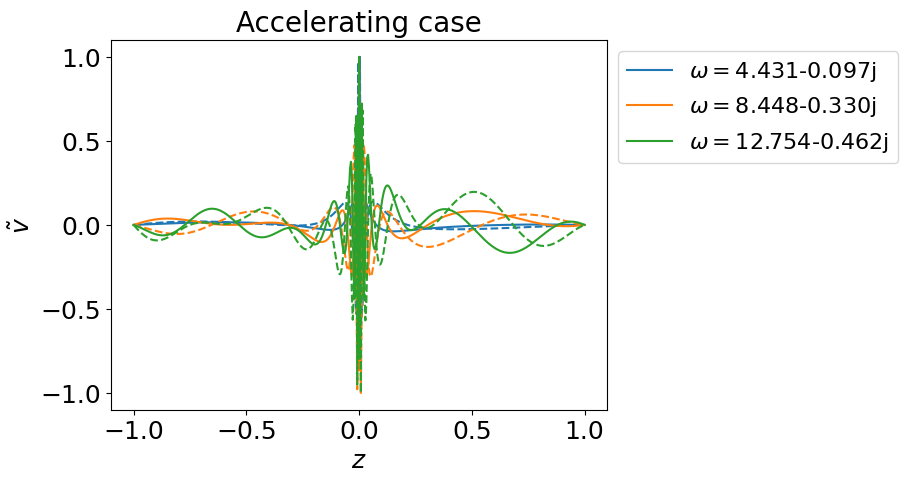
\includegraphics[width=0.95\textwidth]{figures/results-bad-accelerating-v.png}
  \end{center}
  \caption{Dirichlet boundary conditions are set at the two ends, all eigenfunctions are squeezed to the singular point.}
  \label{fig:bad-accelerating-v}
\end{figure}


\end{frame}

\begin{frame}{Interesting Connection to Black Hole}
 \begin{itemize}
  \item The sonic horizon is an exact sonic analogue of black hole horizon. \cite{unruh_sonic_1995}
  \item A quasi-1D fluid flow is ruled by \cite{da_rocha_black_2017}
 \end{itemize}
\begin{align} \label{eq:euler-lagrange}
  \pdv{t}(\rho A) + \pdv{x}(\rho A v) &= 0 \\
  \pdv{t}(\rho A v) + \pdv{x}[(\rho v^2 + p)A] &= 0 \\
  \pdv{t}\left(\frac{\rho v^2}{2} - \frac{p}{1-\gamma}A\right) +
  \pdv{x}\left[ \left(\frac{\rho v^2}{2} - \frac{\gamma}{1-\gamma}A\right)Av \right] &= 0
\end{align}

In \cite{da_rocha_black_2017, furuhashi_simulation_2006}, the acoustic analogue of tortoise coordinate is used to transform the above to Schr{\"o}dinger-type equation,
\[ x^* = c_{s0}\int [c_s(x)(1-M(x)^2)]^{-1} dx \]
where $c_{s0}$ denotes the stagnation speed of sound, $c_s = \dv*{p}{\rho}$ is the local speed of sound and $M(x)= v(x)/c_s(x)$ is the Mach number.
\end{frame}

\begin{frame}{Shooting Method}
  \begin{itemize}
    \item Employed shooting method.
    \item Expanded $\tilde{v}$ near singularity.
    \item Picked up regular solution.
    \item Shoot regular solution to the left and match boundary condition.
  \end{itemize}
  \begin{figure}[htbp]
    \begin{center}
      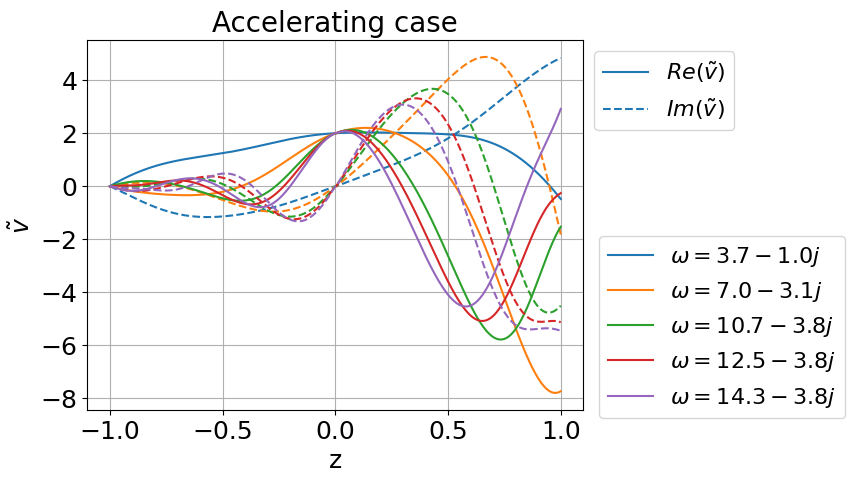
\includegraphics[width=0.7\textwidth]{figures/results-accelerating-v.png}
    \end{center}
    \caption{The solutions crosses the singular point smoothly. All modes are stable.}
    \label{fig:good-accelerating-v}
  \end{figure}
\end{frame}
